% Declare Document Class
\documentclass[a4paper,12pt,twoside,twocolumn]{book}

	% Latex Packages
\usepackage[T1]{fontenc}
\usepackage[utf8]{inputenc}
\usepackage{lmodern}
\usepackage{geometry}
\usepackage{listings}
\usepackage{color}
\usepackage[usenames,dvipsnames,svgnames]{xcolor}
\usepackage{graphicx}
\usepackage[numbers,square,sectionbib,comma,nonamebreak,elide]{natbib}
\usepackage{float}
\usepackage[english]{babel}
\usepackage{fancyhdr}
\usepackage{wrapfig}
\usepackage{array}
\usepackage{lipsum}
\usepackage{fancybox}
\usepackage{varwidth}
\usepackage{enumitem}
\usepackage{titlepic}
\usepackage[nottoc]{tocbibind}
\usepackage{url}
\usepackage[showisoZ]{datetime2}
\usepackage{transparent}
\usepackage{soul}
\usepackage{caption}
\usepackage{enumitem}
\usepackage{amssymb}
\usepackage{tikzsymbols} % http://ctan.math.utah.edu/ctan/tex-archive/graphics/pgf/contrib/tikzsymbols/tikzsymbols.pdf
\usepackage{textcomp}
\usepackage{parskip}
\usepackage{fourier}
\usepackage{array}
\usepackage{makecell}
\usepackage{inconsolata} 
\usepackage{blindtext}
\usepackage{expdlist} 
\usepackage{epigraph} % used to style quotes
\usepackage{titling} % makes available \thetitle \theauthor \thedate
\usepackage[toc,acronym,footnote,nomain]{glossaries} % Load the package with the acronym option
\usepackage{chngcntr}
\usepackage[unicode=false,
    colorlinks=true,
    linkcolor=darkgray,
    citecolor=darkgray,
    filecolor=darkgray,
    urlcolor=darkgray]{hyperref} % https://en.wikibooks.org/wiki/LaTeX/Hyperlinks


\catcode`\_=12


% styles list is available at
% https://www.sharelatex.com/learn/Natbib_bibliography_styles
\bibliographystyle{unsrtnat}


% Path where images are located relative
% to the file main.tex
\graphicspath{{img/}{figures/}}


% In which order to look after images in
% declared graphicspath{}'s
% 1. Low-quality JPG
% 2. Med-quality PNG
% 3. High-quality PDF
\DeclareGraphicsExtensions{.jpg,.png,.pdf}


\fancypagestyle{fancybook}{%
	\fancyhf{}%
	% Note the ## here. It's required because \fancypagestyle is making a macro (\ps@fancybook).
	% If we just wrote #1, TeX would think that it's the argument to \ps@fancybook, but
	% \ps@fancybook doesn't take any arguments, so TeX would complain with an error message.
	% You are not expected to understand this.
	\renewcommand*{\sectionmark}[1]{ \markright{\thesection\ ##1} }%
	\renewcommand*{\chaptermark}[1]{ \markboth{\chaptername\ \thechapter: ##1}{} }%
	% Increase the length of the header such that the folios 
	% (typography jargon for page numbers) move into the margin
	\fancyhfoffset[LE]{6mm}% slightly less than 0.25in
	\fancyhfoffset[RO]{6mm}%
	% Put some space and a vertical bar between the folio and the rest of the header
	\fancyhead[LE]{\color{GreenYellow}\thepage\hskip3mm\vrule\hskip3mm\leftmark}%
	\fancyhead[RO]{\color{GreenYellow}\rightmark\hskip3mm\vrule\hskip3mm\thepage}%
}
\pagestyle{fancybook}


% Use the roman numeric system for pagenumbers
\pagenumbering{roman}


% Usage: \pic[<pct-of-columnwidth>]{<path-to-file>}
\newcommand{\pic}[2][50]{
\begin{center}
    \transparent{0.4}
    \includegraphics[width=0.#1\columnwidth]{#2}
\end{center}
}

% Usage: \fig{<path-to-file>}{<label>}{<caption>}
\newcommand{\fig}[4]{
\begin{figure}[h!]
    \centering
    \includegraphics[width=0.95\columnwidth]{#1}
    \caption{#3}
    \label{fig:#2}
\end{figure}
}

% Usage: \svg{<path-to-file>}{<label>}{<caption>}
\newcommand{\svg}[3]{
    \begin{figure}[h]
        \centering
        \includesvg{#1}
        \caption{#3}
        \label{fig:#2}
    \end{figure}
}

\newcommand{\notice}[2]{%
    \shadowbox{%
        \begin{varwidth}{0.85\linewidth}
            \texttt{\textbf{#1}}\\
            #2
        \end{varwidth}
    }
}

\newcommand{\cliline}[2][]{\lstinline[columns=fixed,#1]{#2}}

\newcommand{\utccurrenttime}[0]{%
	\today%
	T%
	\DTMcurrenttime%
	\DTMfetchTZhour{now}%
	:%
	\DTMfetchTZminute{now}
} % Import user-defined commands


\definecolor{codegreen}{rgb}{0,0.6,0}
\definecolor{codegray}{rgb}{0.5,0.5,0.5}
\definecolor{codepurple}{rgb}{0.58,0,0.82}
\definecolor{backcolour}{rgb}{0.95,0.95,0.92}
 %user-defined colors


% https://tex.stackexchange.com/a/174553
\lstdefinestyle{mystyle}{
    language=cisco,
    backgroundcolor=\color{backcolour},
    commentstyle=\color{codegreen}\ttfamily,
    keywordstyle=\color{magenta},
    numberstyle=\tiny\color{codegray},
    stringstyle=\color{codepurple},
    basicstyle=\scriptsize\ttfamily,
    breakatwhitespace=false,
    breaklines=true,
    captionpos=b,
    keepspaces=true,
    numbers=left,
    showspaces=false,
    showstringspaces=false,
    showtabs=false,
    tabsize=4,
    abovecaptionskip=1em,
    aboveskip=1em,
    belowcaptionskip=1em,
    belowskip=3em,
    upquote=true,
    numbersep=8pt,
    rulecolor=\color{black},
}


\lstdefinestyle{plaintxt}{
    language=TeX,
    numbers=none,
    frame=trBL,
    frameround=fttt,
    backgroundcolor=\color{white},
    boxpos=c,
}


\lstdefinelanguage{cisco}{
    keywords={
        access-list,
        cdp,
        dhcp,
        end,
        hostname,
        interface,
        ip,
        line,
        lldp,
        login,
        network,
        no,
        ntp,
        router,
        show,
        shutdown,
        snmp-server,
        vlan,
        vrf
    },
    keywordstyle=\color{blue}\bfseries,
    ndkeywords={
        access-group,
        addr,
        address,
        aux,
        bgp,
        console,
        dhcp,
        eigrp,
        enable,
        fa,
        FastEthernet,
        gi,
        GigabitEthernet,
        group,
        host,
        ifindex,
        isis,
        ospf,
        ospfv3,
        pool,
        rip,
        run,
        view,
        vty
    },
    ndkeywordstyle=\color{darkgray}\bfseries,
    identifierstyle=\color{black},
    sensitive=false,
    comment=[l]{!},
    commentstyle=\color{purple}\ttfamily,
    stringstyle=\color{red}\ttfamily,
    caption=\lstname,
    tabsize=1,
    captionpos=t,
    showstringspaces=false,
    breaklines=true,
    breakatwhitespace=true,    
}


\geometry{a4paper,margin=1.5cm}
\setlength{\columnsep}{1.5cm} %space between columns
\setlength{\headheight}{15pt}
\setlength{\footnotesep}{0.5cm} %space between footnotes:
\setlength{\skip\footins}{2cm} %space between the text body and the footnotes
\setlist[itemize,1]{leftmargin=\dimexpr 26pt-.2cm}
\setlist[itemize,2]{leftmargin=\dimexpr 26pt-.3cm}
\lstset{style=mystyle} %apply lst styling


\renewcommand{\familydefault}{\sfdefault}


\DeclareCaptionFormat{myformat}{%
    % #1: label (e.g. "Table 1")
    % #2: separator (e.g. ": ")
    % #3: caption text
    \begin{varwidth}{\linewidth}%
        \centering
        #1#2#3%
    \end{varwidth}%
}
\captionsetup{format=myformat}% global activation


\newlist{todolist}{itemize}{2}
\setlist[todolist]{label=$\square$}
\usepackage{pifont}
\newcommand{\cmark}{\ding{51}}%
\newcommand{\xmark}{\ding{55}}%
\newcommand{\done}{\rlap{$\square$}{\raisebox{2pt}{\large\hspace{1pt}\cmark}}%
    \hspace{-2.5pt}}
\newcommand{\wontfix}{\rlap{$\square$}{\large\hspace{1pt}\xmark}}


\renewcommand\theadalign{cb}
\renewcommand\theadfont{\bfseries}
\renewcommand\theadgape{\Gape[4pt]}
\renewcommand\cellgape{\Gape[4pt]}

\def\tsq#1{\textquotesingle{#1}}
\def\bsq#1{%both single quotes
    \lq{#1}\rq}


\makeglossaries % Generate the glossary


\renewcommand*{\acronymname}{Abbreviations}


% Do not reset counter for footnotes at all
% through the document from start to finish.
% https://tex.stackexchange.com/a/10449
\counterwithout{footnote}{chapter}


% Do not reset counter for figures at all
% through the document from start to finish.
% https://tex.stackexchange.com/a/28334
\counterwithout{figure}{chapter}


% Set footnote numeration
% https://www.sharelatex.com/learn/Footnotes
% This command need to be run AFTER
% "\counterwithout{footnote}{chapter}" for the
% changes to be able to take effect.
\renewcommand{\thefootnote}{\arabic{footnote}}


\addtolength{\skip\footins}{2pt}    % vertical space between rule and main text


% https://tex.stackexchange.com/a/141975
\let\origfootnote\footnote % font size of footnotes; changes \footnotesize command only inside footnotes!
\renewcommand{\footnote}[1]{%
    \renewcommand\footnotesize\scriptsize % here there is scriptsize in footnotes (example)       
    \origfootnote{#1}}
 % Load structure cfg for document

%%%%%%%%%%%%%%%%%%%%%%%%%%%%%%%%%%%%%%%%%%%%%%%%%%%%%%
%                                                    %
% BEGIN DOCUMENT                                     %
%                                                    %
%%%%%%%%%%%%%%%%%%%%%%%%%%%%%%%%%%%%%%%%%%%%%%%%%%%%%%

\begin{document}

% Which info to insert on the title page
\title{r17dinh409}
\author{Christoffer Hansen <zbcchhan11 at zbc.dk>}
\date{May 22 - June 30, 2017}
\titlepic{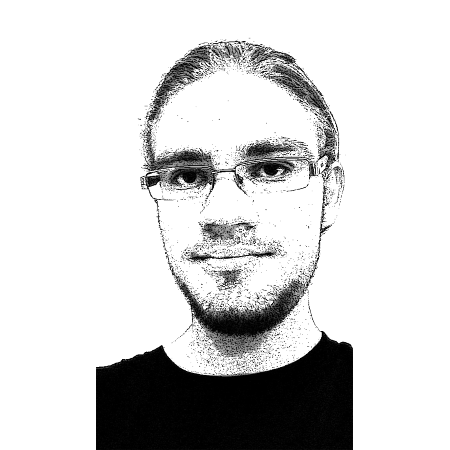
\includegraphics[width=0.3\textwidth]{profilepic/pic1}}
\maketitle

\tableofcontents

%\setlength{\parindent}{4em}

% Define length between paragrahps
\setlength{\parskip}{0.35em}

% Define lineheight
\renewcommand{\baselinestretch}{1.15}

%%%%%%%%%%%%%%%%%%%%%%%%%%%%%%%%%%%%%%%%%%%%%%%%%%%%%%
%                                                    %
% BEGIN CHAPTER: Base Configuration                  %
%                                                    %
%%%%%%%%%%%%%%%%%%%%%%%%%%%%%%%%%%%%%%%%%%%%%%%%%%%%%%

\chapter{Base Configuration}

\section{Cisco Lab}

% <!-- ROUTER -->

\subsection{Router}
\subsubsection{File: base.cfg}
%\lstinputlisting[language=tcl]{code/router/base.cfg}
\subsubsection{File: reset.tcl}
%\lstinputlisting[language=tcl]{code/router/reset.tcl}

\newpage

% <!-- LAYER 3 SWITCH -->

\subsection{Layer 3 Switch}
\subsubsection{FILE: base.cfg}
\lstinputlisting[language=tcl]{code/l3switch/base.cfg}
\subsubsection{FILE: reset.tcl}
\lstinputlisting[language=tcl]{code/l3switch/reset-tcl.txt}
\subsubsection{FILE: resetvlans.tcl}
\lstinputlisting[language=tcl]{code/l3switch/resetvlans-tcl.txt}

\newpage

% <!-- LAYER 2 SWITCH -->

\subsection{Layer 2 Switch}
\subsubsection{FILE: base.cfg}
\lstinputlisting[language=tcl]{code/l2switch/base.cfg}
\subsubsection{FILE: reset.tcl}
\lstinputlisting[language=tcl]{code/l2switch/reset-tcl.txt}
\subsubsection{FILE: resetvlans.tcl}
\lstinputlisting[language=tcl]{code/l2switch/resetvlans-tcl.txt}

%%%%%%%%%%%%%%%%%%%%%%%%%%%%%%%%%%%%%%%%%%%%%%%%%%%%%%
%                                                    %
% BEGIN CHAPTER: Protocols                           %
%                                                    %
%%%%%%%%%%%%%%%%%%%%%%%%%%%%%%%%%%%%%%%%%%%%%%%%%%%%%%

\chapter{Protocols}

\section{Routed Network}

\subsection{OSPF}
\subsection{IS-IS}
\subsection{EIGRP}
\subsection{RIP}
\subsection{Static}
\subsection{BGP}

\newpage

\section{Switch Network}

\subsection{VTP}
\fig{vtp/implementing-vtp}{imp-vtp1}{VTP}

\subsubsection{VTP Modes}
The tree modes a VTP \textit{enabled} device can operate are
\begin{itemize}
    \item Transparent
    \item Server
    \item Client
\end{itemize}
Of course you can \textit{disable} VTP altogether.

Key things to be aware of \textit{before} enabling VTP in your environment is to make double sure of only having 1 VTP domain. \textbf{If} 2 or more VTP domains exists. Be triple sure to separate them! As to avoid having an VTP server DB overridden with data from another VTP domain.

The three VTP modes \textit{operates} as follow
\begin{itemize}
    \item Transparent
    \begin{itemize}
        \item Creates, modifies and deletes \textit{local} vlans only
        \item Forwards advertisements
        \item Does \textit{not} synchronizes vlan configurations.
    \end{itemize}
    \item Server
    \begin{itemize}
        \item Creates, modifies and deletes vlans
        \item Sends and forwards advertisements
        \item Synchronizes vlan configurations
    \end{itemize}
    \begin{itemize}
        \item Cannot create, modify or delete vlans
        \item Send and forwards advertisements
        \item Synchronizes vlan configurations
    \end{itemize}
\end{itemize}

\subsubsection{VTP Announcement}
VTP operates with announcements sent out in intervals. Summarized it amounts to
\begin{itemize}
    \item 1 \textit{summary} announcement per 5th minute from the server
    \item The summary announcement informs clients of the current revision
    \item An announcement is sent out \textit{on the spot} when a change has been made on the VTP server
\end{itemize}

Do remember it is \textbf{only} the VTP server which has the vlan configuration stored \textbf{on disk}. All device clients and transparent nodes do only store the vlans delegated by VTP in memory.

\subsubsection{Common Issues}
\begin{itemize}
    \item Different/Incompatible VTP versions
    \item Wrong password
    \item Incorrect mode name
    \item No server set (all devices configured in transparent/client/vtp disabled mode)
\end{itemize}

\subsubsection{VTP Versions}
\begin{itemize}
    \item Version 1
    \item Version 2
    \begin{itemize}
        \item Version-dependent	transparent	mode
        \item Consistencycheck
        \item Token ring support
        \item Unrecognized type-length-value support
    \end{itemize}
    \item Version 3 (not "yet" common)
    \begin{itemize}
        \item Extended VLAN support: Allow ranges are 1-1005,1018-2095. Not mentioned vlans ranges up to 4095 is still reserved.
        \item Domain name is not automatically learned.
        \item Better security.
        \item Better database propagation.
        \item MST now supported.
    \end{itemize}
\end{itemize}

\subsubsection{VTP Pruning}
The art of only allowing the vlan traffic to flow on \textit{necessary} links.

This means if there are no clients in a vlan on a device. Then no traffic for the inactive vlans is send down-/upstream on the link in question.
\fig{vtp/vtp-pruning}{vtpruning1}{VTP Pruning}

\subsubsection{Security}
It is \textbf{strongly} recommended to enable the security features supported in VTP.

\textbf{Password:} MD5 hashing, Case-sensitive, Length between 8 and 64 chars.

\notice{VTP Scaling}{
As the network grows and grows and grows and grows some more over long/short timespans.
You will \textbf{for certain} come to cross-rode, where you \textbf{must} consider to
go away from using VTP in the network. The problems of managing an elderly network and
wiping and re-introducing nodes in the network. You \textbf{will} face the issue of a
wiped vlan database from the VTP domain.
}

\subsubsection{Example configuration}
\lstinputlisting{code/vtp/example.cfg}

\subsection{Channel Bundling (aka. EtherChannel, PortChannel)}
Channel bundling is the "art" of using multiple physical links as one single logical link in when viewed from the perspective of the forwarding plane.

Technologies:
\begin{itemize}
    \item \textbf{PAgP:} The Cisco-only thingy
    \item \textbf{LACP:} The IEEE standard
    \item \textbf{Static:} Just forced on
\end{itemize}

\fig{channelbundling/network-without-channelbundling}{noethernetchannel}%
{No Channelbundling present}

Channel bundling of switch ports in the network may or may not be the best idea, in regards to the networks growth rate in terms of min. required bandwidth.

Channel bundling spreads out the in and egress flows based upon one of several methods configured on the switch:
\begin{itemize}
    \item Source to Destination MAC
    \item Source to Destination IP
\end{itemize}
Keep in mind this will by no means archive true load balancing. Where all links are equally used based upon number of flows \textit{or} in terms of used bandwidth.

\begin{table}[h]
    \centering
    \caption{Channel bundling mechanisms}
    \label{chbundmech1}
    \resizebox{\columnwidth}{!}{%
        \begin{tabular}{|l|l|l|}
            \hline
            Hash Input Code & Hash Input Detecision & Switch Model \\ \hline
            dst-ip          & Dest IP addr          & All models   \\ \hline
            dst-mac         & Dest MAC addr         & All models   \\ \hline
            src-dst-ip      & Src and dest IP addr  & All models   \\ \hline
            src-dst-mac     & Src and dest MAC addr & All models   \\ \hline
            src-ip          & Src IP addr           & All models   \\ \hline
            src-mac         & Src MAC addr          & All models   \\ \hline
            src-port        & Src port no           & 4500,6500    \\ \hline
            dst-port        & Dest port no          & 4500,6500    \\ \hline
            src-dst-port    & Src and dest port no  & 4500,6500    \\ \hline
        \end{tabular}%
    }
\end{table}

\fig{channelbundling/network-with-channelbundling}{withethernetchannel}%
{Channelbundling present}

\subsubsection{Protocol Properties}

\begin{itemize}
    \item LACP
    \begin{itemize}
        \item Active: Enabled
        \item Passive: Waits for LACP packets on the wire before enabled
    \end{itemize}
    \item PAgP
    \begin{itemize}
        \item Desirable: Enabled
        \item Auto: Waits for PAgP packets on the wire before enabled
    \end{itemize}
\end{itemize}

Some other \underline{required} settings to be (equal across all ports) aware of when configuring Channel bundling are
\begin{enumerate}
    \item Port speeds
    \item Duplex mode
    \item Configured vlan ranges
\end{enumerate}

\subsubsection{Example configuration}
\lstinputlisting{code/channelbundling/example.cfg}

%%%%%%%%%%%%%%%%%%%%%%%%%%%%%%%%%%%%%%%%%%%%%%%%%%%%%%
%                                                    %
% BEGIN section: Spanning Tree                       %
%                                                    %
%%%%%%%%%%%%%%%%%%%%%%%%%%%%%%%%%%%%%%%%%%%%%%%%%%%%%%

\newpage
\section{Spanning Tree}

Spanning Tree exists for the \textbf{sole} reason to save "your" network and all the broadcast storms an network engineer having a bad day can by mistake create!

STP comes from the above desire where redundancy was wanted but no protocol existed before STP to help in this regard.

\begin{table}[h]
	\centering
	\caption{Spanning Tree standrds}
	\label{stpstandards}
	\resizebox{\columnwidth}{!}{%
		\begin{tabular}{|l|l|l|l|l|}
			\hline
			\textbf{} & \textbf{Standard} & \textbf{Ressource Usage} & \multicolumn{2}{l|}{\textbf{Convergence}} \\ \hline
			CST       & 802.1D            & Low                      & Slow              & All vlans             \\ \hline
			PVST+     & Cisco             & High                     & Slow              & Per vlan              \\ \hline
			RSTP      & 802.1w            & So-so (Med.)             & Fast              & All vlans             \\ \hline
			RPVST+    & Cisco             & On-the-double (V.High)   & Fast              & Per vlan              \\ \hline
			MST       & 802.1s            & Med. - High              & Fast              & Vlan list             \\ \hline
		\end{tabular}%
	}
\end{table}

\subsection{Port Roles}

When a switch is enabled for Spanning Tree. One of the following roles will have been assumed by any port on the switch in question.

\begin{itemize}
	\item \textbf{Root port:} Only 1 port on any switch (non-counting the root bridge!). Is always the port with the lowest metric (aka. best path) to the root bridge.
	\item \textbf{Designated port:} A designated port is the port on any segment closest to the root bridge and forwarding traffic.
	\item \textbf{\textit{Non}-designated port:} Put in blocking mode and not currently forwarding traffic.
	\item \textbf{Disabled port:} The port has been one-way-or-another shut down.
\end{itemize}

\subsection{Standards}

\subsubsection{STP}

\subsubsection{PVST}

\subsubsection{RPVST+}

\subsubsection{MST}

\subsection{Features}

\begin{itemize}
	\item PortFart
	\item UplinkFast
	\item BackboneFast
	\item BPDU Guard
	\item BPDU Filter
	\item Root Guard
	\item Loop Guard
	\item Unidirectional Link Detection (UDLD)
	\item FlexLinks
\end{itemize}

%%%%%%%%%%%%%%%%%%%%%%%%%%%%%%%%%%%%%%%%%%%%%%%%%%%%%%
%                                                    %
% BEGIN CHAPTER: Internet                            %
%                                                    %
%%%%%%%%%%%%%%%%%%%%%%%%%%%%%%%%%%%%%%%%%%%%%%%%%%%%%%

\chapter{Internet}

\section{BGP}

%%%%%%%%%%%%%%%%%%%%%%%%%%%%%%%%%%%%%%%%%%%%%%%%%%%%%%
%                                                    %
% BEGIN LIST OF FIGURES                              %
%                                                    %
%%%%%%%%%%%%%%%%%%%%%%%%%%%%%%%%%%%%%%%%%%%%%%%%%%%%%%

\renewcommand{\listfigurename}{List of {\footnotesize hidden} Figures}
\listoffigures

%%%%%%%%%%%%%%%%%%%%%%%%%%%%%%%%%%%%%%%%%%%%%%%%%%%%%%
%                                                    %
% BEGIN LIST OF TABLES                               %
%                                                    %
%%%%%%%%%%%%%%%%%%%%%%%%%%%%%%%%%%%%%%%%%%%%%%%%%%%%%%

\renewcommand{\listtablename}{Tables {\footnotesize hidding} on the pages}
\listoftables

%%%%%%%%%%%%%%%%%%%%%%%%%%%%%%%%%%%%%%%%%%%%%%%%%%%%%%
%                                                    %
% BEGIN REFERENCES                                   %
%                                                    %
%%%%%%%%%%%%%%%%%%%%%%%%%%%%%%%%%%%%%%%%%%%%%%%%%%%%%%

\bibliographystyle{unsrt}
\bibliography{unsrt}

%%%%%%%%%%%%%%%%%%%%%%%%%%%%%%%%%%%%%%%%%%%%%%%%%%%%%%
%                                                    %
% END DOCUMENT                                       %
%                                                    %
%%%%%%%%%%%%%%%%%%%%%%%%%%%%%%%%%%%%%%%%%%%%%%%%%%%%%%

\end{document}
